\chapter{Travail effectué par Thibaud LE DOLEDEC et Clément AILLOUD}

\section{Driver de la centrale inertielle (IMU)}

Clément AILLOUD a développé un driver Linux pour la centrale inertielle en utilisant le framework \codeinline{text}{iio}. Celui-ci supporte actuellement le gyroscope et l'accéléromètre mais pas le magnétomètre. Il est compatible avec les bus I2C et SPI. Sur l'Autoscope, le bus I2C sera utilisé.

Un patch du device tree permettant le support du driver est également fourni.

\vspace{1cm}

Le driver a été intégré au système d'exploitation du télescope. \codeinline{text}{iio} permet d'accéder aux données issues de l'IMU via le dossier suivant~:

\code{text}
root@autoscope ~ #
    ls /sys/bus/iio/devices/iio:device0/
        dev               in_accel_y_raw    in_anglvel_x_raw  in_temp_input  power
        in_accel_scale    in_accel_z_raw    in_anglvel_y_raw  name           subsystem
        in_accel_x_raw    in_anglvel_scale  in_anglvel_z_raw  of_node        uevent

    cat /sys/bus/iio/devices/iio:device0/name
        mpu9250-i2c
\end{minted}

\section{Interface utilisateur (Plugin de Stellarium)}

Le logiciel Stellarium offre la possibilité de développer des plugins aux fonctionnalités diverses. Nous avons décidé d'utiliser un plugin pour faire de Stellarium l'élément principal de l'interface utilisateur du télescope.

\vspace{1cm}

Thibaud LE DOLEDEC a développé un plugin de Stellarium permettant les actions suivantes~:
\begin{itemize}[label=$\bullet$]
	\item Rechercher un astre et le suivre tant à l'écran qu'avec le télescope (par l'envoi régulier de coordonnées spatiales à celui-ci).
	\item Demander au télescope ses coordonnées de position et de visée et afficher la vue du ciel simulé correspondante.
	\item Ordonner au télescope de prendre une photo. Il existe une interface destinée à configurer les paramètres de la caméra (temps d'exposition, etc.).
	\item Se connecter au serveur FTP du télescope pour récupérer les clichés du ciel.
	\item Afficher un aperçu de ce que voit le télescope à l'instant présent (retransmission d'un flux vidéo). Un espace actuellement matérialisé par un rectangle gris est destiné à cela.
	\end{itemize}

\vspace{1cm}

\begin{figure}[H]
    \centering
    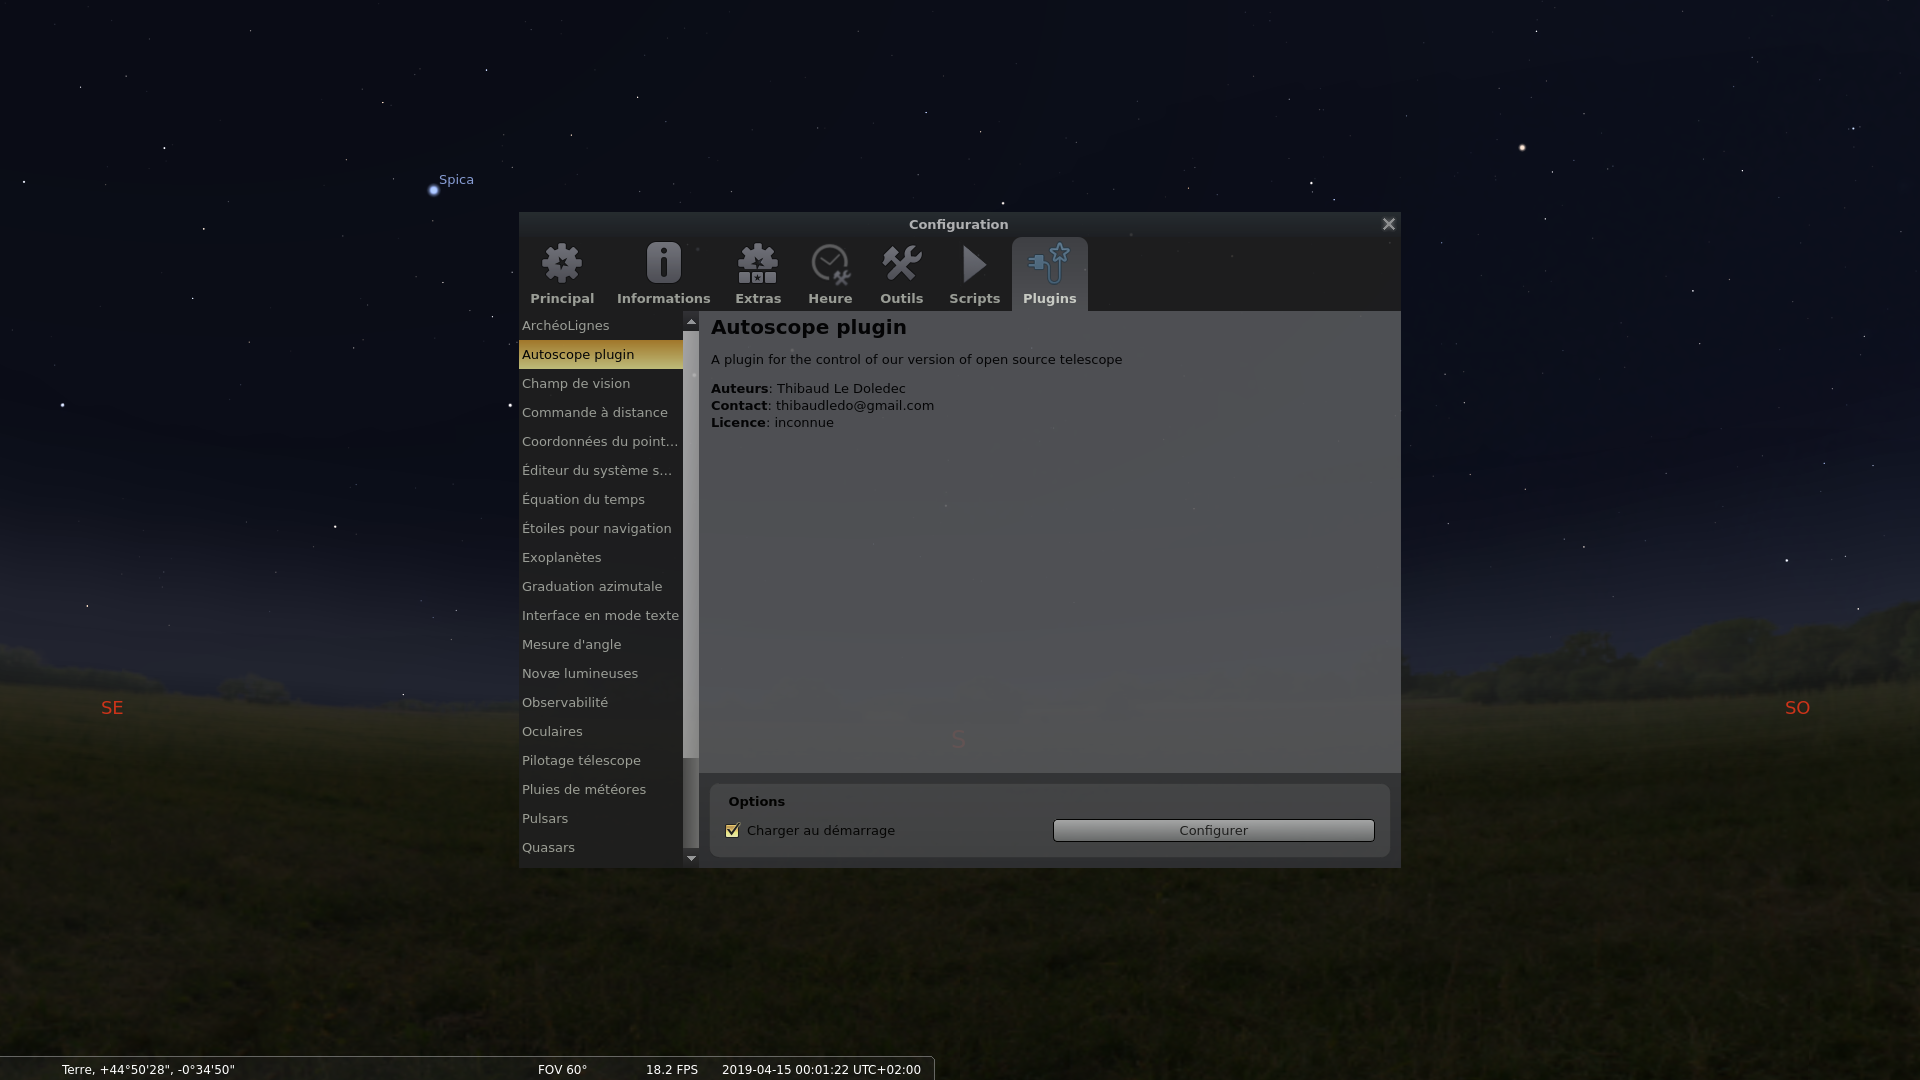
\includegraphics[width=0.9\linewidth]{\figures/photo_stellarium_3.png}
    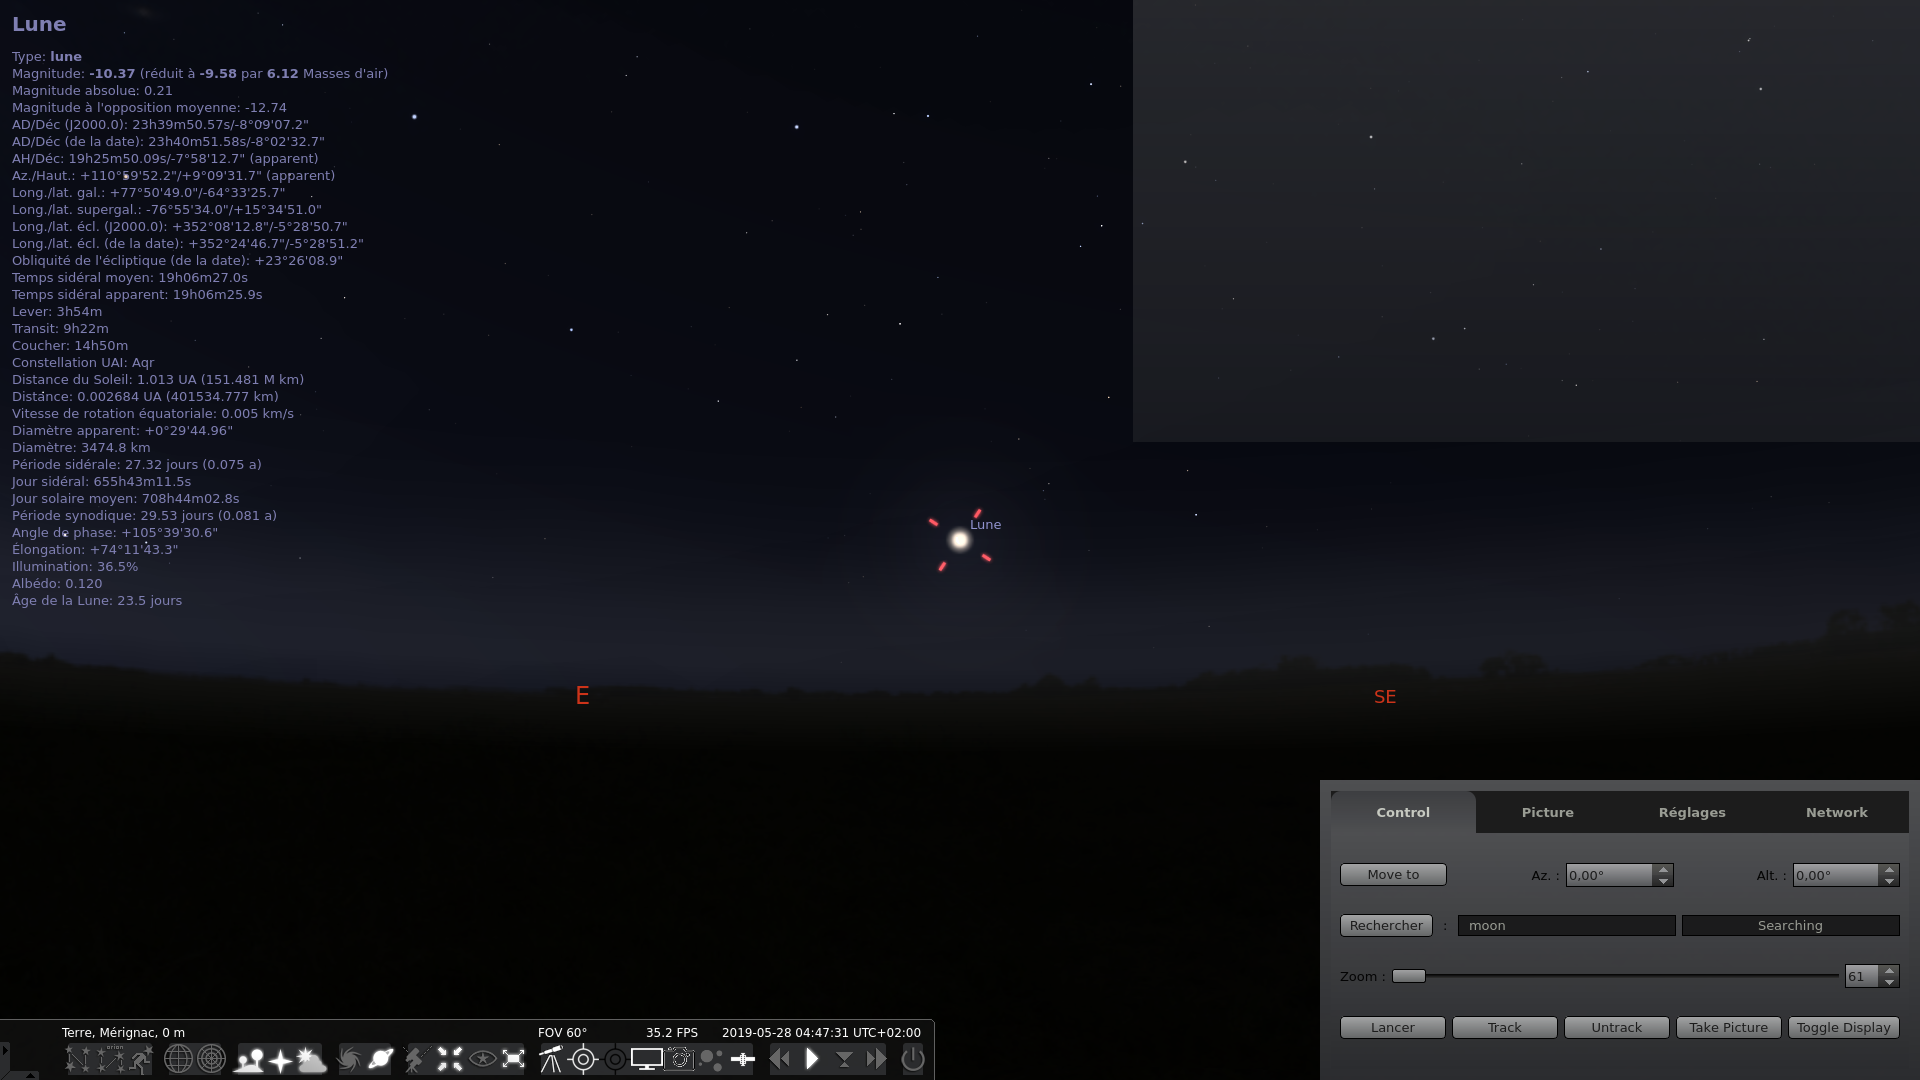
\includegraphics[width=0.9\linewidth]{\figures/photo_stellarium_4.png}
    \decoRule
    \caption[
    Aperçu de l'interface du plugin de Stellarium]{
    Aperçu de l'interface du plugin de Stellarium}
    \label{fig:Aperçu de l'interface du plugin de Stellarium}
    \end{figure}

\vspace{1cm}

Le plugin fonctionne correctement, bien que certains éléments soient sûrement à retravailler lors du développement du logiciel principal du télescope.

La gestion de la communication FTP repose sur l'utilisation d'une librairie dépréciée \codeinline{text}{qtftp} qui a semblé poser problème lors des essais de déploiement du travail réalisé par Thibaud. L'idéal serait de se passer de cette librairie.

\vspace{1cm}

Thibaud et Clément ont rédigé un document disponible à l'adresse suivante qui explique la procédure à suivre pour développer un plugin de Stellarium.
\url{https://github.com/thibaudledo/Autoscope/blob/latex/Tutoriel_Stellarium.pdf}
